\chapter{Grundlagen}
\label{chap:voraussetzungen}
Dieses Kapitel soll oberflächlich einige Dinge erklären, die für diese Arbeit vorausgesetzt werden.
\section{Git}
Als \Gls{vcs} setzen wir Git ein. Ins Git gehört jeglicher entwickelte Code, nicht aber Artefakte (gebuildeter Code) und IDE spezifische Einstellungen. Die entsprechenden Verzeichnisse müssen wir also in die \ctexttt{.gitignore}-Datei aufnehmen. Wir werden verschiedene Git Repositories verwenden für die verschiedenen Teilgebiete des Roboters, also die Domänen. Die Domänen sind wie in nachfolgender Tabelle \ref{tab:gitRepositories} unterteilt:
\begin{table}[H]
	\centering
	\begin{tabular}{lp{13cm}} \toprule
		\textbf{Repository}          & \textbf{Beschreibung}\\ \midrule
		\texttt{robocup-parent-pom}  & Unser projektweites Parent-POM \\ \midrule
		\texttt{robocup-common}      & Alles, was übergreifend im ganzen Robocup-Projekt gemeinsam ist. Bis jetzt vor allem statische Strings zum verwenden und Ressourcen.\\ \midrule
		\texttt{robocup-connectors}  & Alle domainübergreifende Servants\\ \midrule
		\texttt{robocup-positioning} & Dinge aus der Domäne Positioning. TiM55x-Service und Hardware-Mock\\ \midrule
		\texttt{robocup-ui}          & UI-spezifisches\\ \bottomrule
	\end{tabular}
	\caption{Übersicht über die Namen der Git-Repositories bzw. der Domänen}
	\label{tab:gitRepositories}
\end{table}

Im Anhang \ref{chap:tranition-git} sind noch einige Dinge festgehalten, die für die Umbauphase bei der HFTM relevant sind.

\section{Apache Maven}
\label{chap:maven}
Maven ist ein Tool um den Build-Prozess von Software zu unterstützen. Es bietet beispielsweise Unterstützung fürs Managen der Abhängigkeiten, fürs Testing und zur Paketierung. Es gibt auch andere Tools, die dazu eingesetzt werden können (Bsp. Gradle). Wir konzentrieren uns hier aber auf Maven, da es in der Software-Entwicklung mit Java aktuell der De-facto-Standard ist. Die zu entwickelnden Services aus Kapitel \ref{chap:beispielimplementation} verwenden Maven vor allem für das Dependency-Management. Konkret ist Maven in diesem Projekt für folgendes zuständig:
\begin{itemize}
	\item
	Libraries müssen nicht manuell heruntergeladen und ins Projekt aufgenommen werden.
	\item
	Versionen der Libraries sind zentral definiert. Ein Upgrade einer Library auf eine neue Version lässt sich somit an einem Ort erledigen.
	\item
	Paketierung der Services/Applikationen als Jar-Datei.
\end{itemize}
Um Maven zu verwendet erstellt man in der verwendeten Entwicklungsumgebung (\acrshort{ide}) ein 'Maven-Projekt'. Zentral in einem Maven-Projekt ist die Datei \texttt{pom.xml} (\acrshort{pom} steht für \acrlong{pom}). Sie definiert wie oben erläutert die Umgebung für das Java-Projekt.

\subsection{Dependencies}
Maven verwendet so genannte Repositores um Libraries anzuziehen. Repositories können vom Typ LOCAL oder REMOTE sein. Wie die Namen vermuten lassen befindet sich ein Lokales Repository auf dem Entwickler-PC und ein Remote Repository im Internet/Netzwerk. Libraries bzw. Dependencies sucht man beispielsweise auf \href{https://mvnrepository.com/}{mvnrepository.com} oder \href{https://search.maven.org}{search.maven.org}, der so genannten 'Maven Central'. Alle Libaries in diesem Repository kennt Maven automatisch und kann diese herunterladen. Heruntergeladen werden die Libraries (als Jar paketiert) in das lokale Repository, also in den Ordner \texttt{.m2} im Home-Verzeichnis des ausführenden Benutzers. In dieser Arbeit ist das also \ctexttt{/home/mkilchhofer/.m2/repository} (Fedora Linux) und unter Windows wird das in \ctexttt{\path{C:\Users\mkilchhofer\.m2\repository}} sein.

Als kurzes Beispiel hier eine Demonstration zur Einbindung von Log4j2.
\begin{enumerate}
	\item Auf mvnrepository nach ,,Log4j Core'' suchen.
	\item Version auswählen (hier zum Beispiel ,,2.11.0'')
	\item XML-Struktur (Abbildung \ref{fig:mvnrepository-example}) im \texttt{pom.xml} in den Sub-Baum \texttt{<dependencies>} einfügen (Listing \ref{lst:maven-example-simple})
\end{enumerate}

\begin{figure}[H]
	\centering
	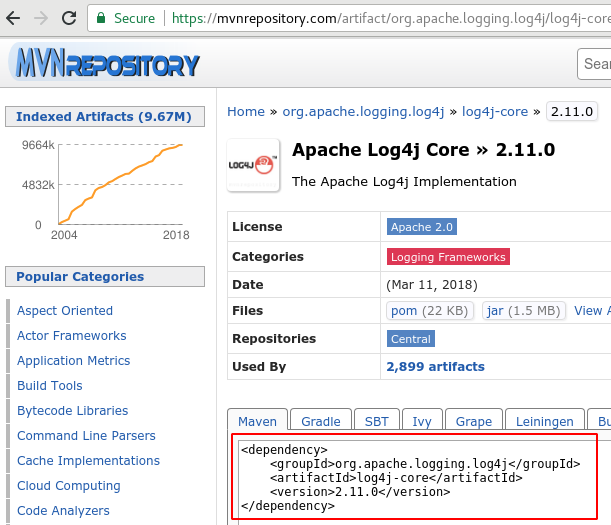
\includegraphics[width=0.7\textwidth]{img/mvnrepository-log4j-example.png}
	\caption{Code zum kopieren von \texttt{mvnrepository.com}}
	\label{fig:mvnrepository-example}
\end{figure}

\begin{lstlisting}[language=XML, caption={Simples Beispiel wie ein pom.xml aussieht},label={lst:maven-example-simple}]
<?xml version="1.0" encoding="UTF-8"?>
<project <!-- (generiert die IDE) --> >
  <modelVersion>4.0.0</modelVersion>
  <artifactId>lidar-hardware-service</artifactId>
  <groupId>info.kilchhofer.bfh</groupId>
  <version>1.1-SNAPSHOT</version>
  <packaging>jar</packaging>

  <dependencies>
    <dependency>
      <groupId>org.apache.logging.log4j</groupId>
      <artifactId>log4j-core</artifactId>
      <version>2.11.0</version>
    </dependency>
  </dependencies>
</project>
\end{lstlisting}
Maven übernimmt dann über die \acrshort{ide} den Rest und lädt das Jar und nötigenfalls die Sources herunter (also ins Lokale Repository).

\subsection{Vererbung und Parent-POM}

Von POMs kann wie auch in Java geerbt werden, auch über mehrere Stufen (Abbildung \ref{fig:grundlagen-pom-vererbung}).
\begin{figure}[H]
	\centering
	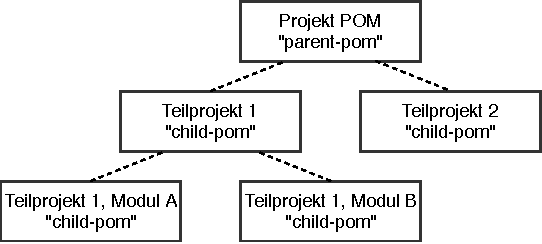
\includegraphics[width=0.5\textwidth]{img/maven-pom-inheritance-generic.pdf}
	\caption{Visualisierung POM Vererbung, generisch}
	\label{fig:grundlagen-pom-vererbung}
\end{figure}
Wo es sinnvoll ist, werden wir also dieses Feature verwenden um Duplizierung in den Teilprojekten zu vermeiden. So wird in diesem Projekt beispielsweise ein Projekt angelegt mit dem Namen ,,robocup-parent-pom''. In diesem POM definieren wir die übergreifenden Dinge. Beispielsweise wollen wir projektweit nur eine Log4j Version unterstützen. Also wird das im Parent-POM wie folgt vorgenommen:
\begin{lstlisting}[language=XML, caption={Ausschnitt aus dem Parent-POM},label={lst:maven-parent-pom}]
<?xml version="1.0" encoding="UTF-8"?>
<project <!-- (generiert die IDE) --> >
  <modelVersion>4.0.0</modelVersion>

  <groupId>info.kilchhofer.bfh</groupId>
  <artifactId>robocup-parent-pom</artifactId>
  <packaging>pom</packaging>
  <version>20180602.4</version>
  <!-- .. not complete -->
  <dependencyManagement>
    <dependencies>
      <!-- .. not complete -->
      <!-- Logging -->
      <dependency>
        <groupId>org.apache.logging.log4j</groupId>
        <artifactId>log4j-core</artifactId>
        <version>2.11.0</version>
      </dependency>
    </dependencies>
  </dependencyManagement>
</project>
\end{lstlisting}

Ein Teilprojekt (Child-POM) kann dies nun wie folgt verwenden ohne die Version zu spezifizieren:
\begin{lstlisting}[language=XML, caption={Ausschnitt aus dem Child-POM},label={lst:maven-child-pom}]
<?xml version="1.0" encoding="UTF-8"?>
<project <!-- (generiert die IDE) --> >
  <parent>
    <groupId>info.kilchhofer.bfh</groupId>
    <artifactId>robocup-parent-pom</artifactId>
    <version>20180602.4</version>
  </parent>
  <modelVersion>4.0.0</modelVersion>

  <groupId>info.kilchhofer.bfh</groupId>
  <artifactId>robocup-common</artifactId>
  <packaging>jar</packaging>
  <version>${revision}</version>
  
  <!-- .. not complete -->
      
  <dependencies>
    <dependency>
      <groupId>org.apache.logging.log4j</groupId>
      <artifactId>log4j-core</artifactId>
    </dependency>
  </dependencies>
</project>
\end{lstlisting}
Das führt uns zu folgender Vererbung der \acrshort{pom}s im Gesamtprojekt:
\begin{figure}[H]
	\centering
	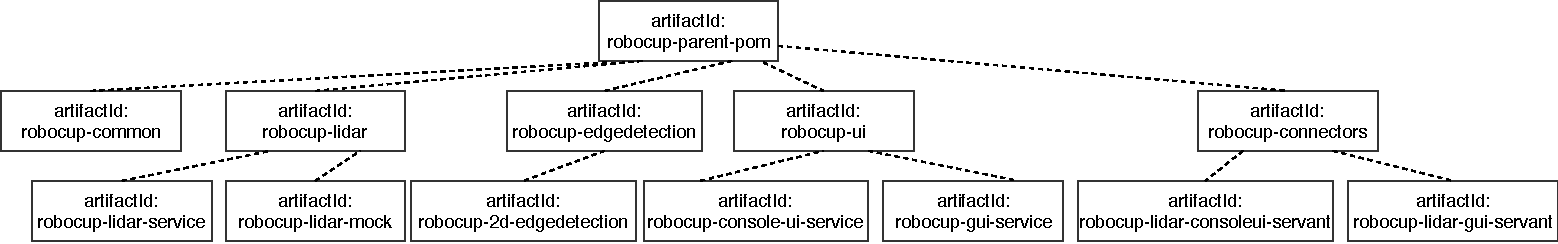
\includegraphics[width=1.0\textwidth]{img/maven-pom-inheritance-robocup.pdf}
	\caption{Visualisierung POM Vererbung in diesem Projekt}
	\label{fig:grundlagen-pom-vererbung-robocup}
\end{figure}


\subsection{Maven Lifecycle}
In jeder aktuellen \acrshort{ide} ist Maven sehr gut eingebunden. So taucht bei einem maven-managed Projekt in der \acrshort{ide} \textit{\Gls{intellij}} folgende Komponente an der rechten Seite auf:
\begin{figure}[H]
	\centering
	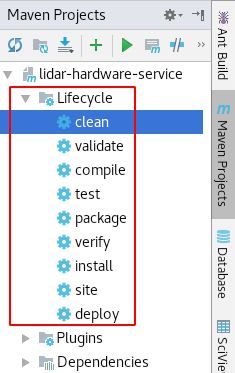
\includegraphics[scale=0.5]{img/maven-lifecycle-ide.png}
	\caption{Maven Lifecycle in der \acrshort{ide}}
	\label{fig:maven-ide}
\end{figure}
Durch das Auswählen der jeweiligen Maven Lifecycle-Phase mit anschliessendem Drücken auf den Play-Knopf wird der entsprechende Task ausgeführt. Was die einzelnen Phasen (Tasks) genau machen ist folgender Tabelle \ref{tab:mavenLifecycle} zu entnehmen.

\begin{table}[H]
	\centering
	\begin{tabular}{lp{13cm}} \toprule
		\textbf{Lifecycle} & \textbf{Beschreibung}\\ \midrule
		\texttt{clean}     & Alle generierten Objekte (namentlich 'Artefakte') und das Verzeichnis \ctexttt{target} werden gelöscht.\\ \midrule
		\texttt{validate}  & Validieren ob alle Projekt-Infos vorhanden und korrekt sind (vor allem pom.xml prüfen).\\ \midrule
		\texttt{compile}   & Kompiliert den Source-Code des Projekts. Syntax-Fehler im Verzeichnis \ctexttt{src/main/..} lassen diese Phase Fehlschlagen. Die Tests aus dem Verzeichnis \ctexttt{src/test/..} werden in dieser Phase noch nicht berücksichtigt. Syntax-Fehler in den Unit-Tests beeinflussen das erfolgreiche Abschliessen dieser Phase nicht.\\ \midrule
		\texttt{test}	   & Führt die Tests gegen den kompilierten Source-Code aus. Diese Tasks endet erfolgreich, wenn die Syntax aller Tests fehlerfrei sind und die Tests erfolgreich durchgeführt werden können.\\ \midrule
		\texttt{package}   & Paketiert den generierten Byte-Code in ein verteilbares Archiv (Bsp. Jar)\\ \midrule
		\texttt{verify}	   & Prüft die paketierten Dateien mittels Integrations-Tests.\\ \midrule
		\texttt{install}   & Kopiert die paketierten Dateien in das lokale Maven Repository (\ctexttt{.m2}-Ordner), um diese als Abhängigkeit in anderen lokalen Projekten zu benutzen.\\ \midrule
		\texttt{site}      & Generiert eine Projekt-Website (heute nicht sehr relevant) \\ \midrule
		\texttt{deploy}	   & Kopiert das generierte Artefakt in ein remote Maven Repository (gleich wie \ctexttt{install}, nur eben Remote. So ist die entwickelte Library auch für andere verfügbar.)				\\ \bottomrule
	\end{tabular}
	\caption{Basic Lifecycle-Phasen in Maven. Quelle: \href{https://maven.apache.org}{maven.apache.org} \cite{maven-build-lifecycle} }
	\label{tab:mavenLifecycle}
\end{table}

\subsection{Build Automatisierung (continuous integration)}
Durch die Verwendung von Maven kann zudem in einem weiteren Schritt der Build-Prozess mit einer Build-Pipeline automatisiert werden. Dies ist möglich, weil im POM alles Nötige spezifiziert ist. Das heisst, wir müssen auf einer neu installierten Umgebung (selbstverständlich mit JDK und Maven vorinstalliert) lediglich folgende Kommandos ausführen und wir haben unsere fertigen Jars:
\begin{lstlisting}[language={none}]
$ git clone <url>/<Unser Git Reposiory>
$ cd <Unser Git Reposiory>
$ mvn clean package
\end{lstlisting}

Die Projekte aus dieser Arbeit verwenden zur Build-Automatisierung \textbf{Travis CI}\footnote{Travis CI: \url{https://travis-ci.org}} und als Ablage bzw. Maven Repository der Artefakte (Jars) \textbf{JFrog Bintray}\footnote{JFrog Bintray: \url{https://bintray.com}}. Wie das ganze konfiguriert wird ist nicht Teil dieser Arbeit, jedoch in den jeweiligen Teil-Projekten in den Dateien \ctexttt{.travis.yml}, \ctexttt{.travis.revision.sh} und \ctexttt{.travis.settings.xml} ersichtlich. \\ Vermutlich werden für den RoboCup sowieso nur Teile davon als Open Source veröffentlicht und deshalb können diese Anbieter nicht unverändert verwendet werden. Beide bieten aber Private Projekte an, die nicht von allen zugänglich sind. Denkbar wäre natürlich auch eine Inhouse-Installation von Jenkins als Build-Automatisierung und JFrog Artifactory OSS als Maven Repository auf einem Server/Notebook/NUC der \acrshort{hftm}.

\section{Tests / Unit Tests}
\label{sec:tests_and_unittests}
Der zu entwickelnde Programmcode soll wie folgt automatisch auf folgenden Stufen getestet werden:
\begin{itemize}
	\item Unit Tests (Klassen und Methoden)
	\item Service-Tests (Tests am API der Servives)
	\item Integrationstests (die verschiedenen Microservices zusammen)
\end{itemize}
Die umgesetzten Tests verwenden JUnit als Framework.  Der Aufbau von JUnit Tests zeigt dieses kleine Beispiel:
\begin{lstlisting}[caption={Simples Beispiel wie JUnit funktioniert},label={lst:junit-example-simple}]
package info.kilchhofer.bfh.lidar.hardwareservice;

import org.junit.jupiter.api.Test;
import static org.junit.jupiter.api.Assertions.assertEquals;
import static org.junit.jupiter.api.Assertions.assertNotEquals;

public class SimpleTest {
	@Test
	@DisplayName("myInt durch 2 teilbar aber nicht durch 3")
	public void mySimpleTest(){
		int myInt = 1024;
		assertEquals(0, (myInt % 2));
		assertNotEquals(0, (myInt % 3));
	}
	
	@Test
	@DisplayName("Log2")
	public void mySimpleTest2(){
		int temp = (int) (Math.log(myInt) / Math.log(2));
		assertEquals(9, temp);
	}
}
\end{lstlisting}
Führt man diesen Test in der \acrshort{ide} \textit{\Gls{intellij}} aus, bekommt man folgenden Output:
\begin{figure}[H]
	\centering
	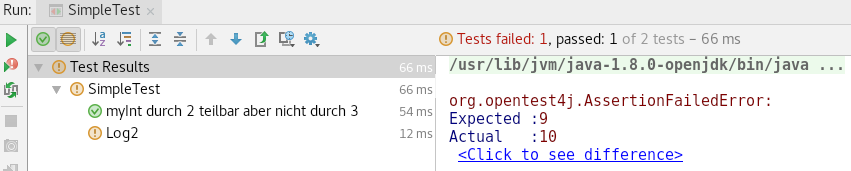
\includegraphics[width=0.7\textwidth]{img/junit-example-ide.png}
	\caption{JUnit Beispieldurchlauf in der \acrshort{ide}}
	\label{fig:junit-example}
\end{figure}
Wie zu erwarten, schlägt der zweite Test fehl, weil der Logarithmus zur Basis 2 von 1024 natürlich 10 ist. Der Erwartungswert im Test ,,Log2'' ist aber 9.

Beispiele die sich auf den entwickelten Code beziehen gibt es im Abschnitt mit der Beispielimplementation (Kapitel \ref{chap:beispielimplementation}).

\section{MQTT}
\label{sec:mqtt}
\acrshort{mqtt} steht für Message Queue Telemetry Transport. Es ist ein leichtgewichtiges Protokoll zum Austausch von Nachrichten über Netzwerke. Es toleriert Netzwerke mit hoher Latenz und schlechter Bandbreite. So wird es häufig für die Machine-to-Machine-Kommunikation (M2M) eingesetzt. Mit Maschine spricht man meist von Sensoren, Aktoren, Mobiltelefonen und embedded Systemen.

\subsection{Publish / Subscribe vs. Request / Response}
\label{sec:publish-subscribe}
Der Unterschied zu den heute weit verbreiteten Microservices mit HTTP ist bei \acrshort{mqtt} das so genannte PubSub-Pattern. Bei diesem Pattern wird nicht wie bei HTTP bei einem Service etwas angefragt, worauf dieser unmittelbar danach eine Antwort gibt (Reqest / Response). Sondern wir abonnieren uns bei einer zentralen Stelle (dem \acrshort{mqtt}-Broker) auf ein bestimmtes Topic (ähnlich einem REST API in der HTTP-Welt) und erhalten je nach Topic erstmals keine Antwort. Sobald jemand (hier ein Service) auf dieses Topic beim \acrshort{mqtt}-Broker Daten publiziert, stellt der Broker diese Nachricht an uns durch. Abonniert man auf ein Topic, auf das zuletzt Daten mit gesetztem "Retain"-Flag im Protokoll-Header publiziert wurden, stellt uns der Broker diese Nachricht unmittelbar nach dem subscribe-Vorgang zu.
\begin{figure}[H]
	\centering
	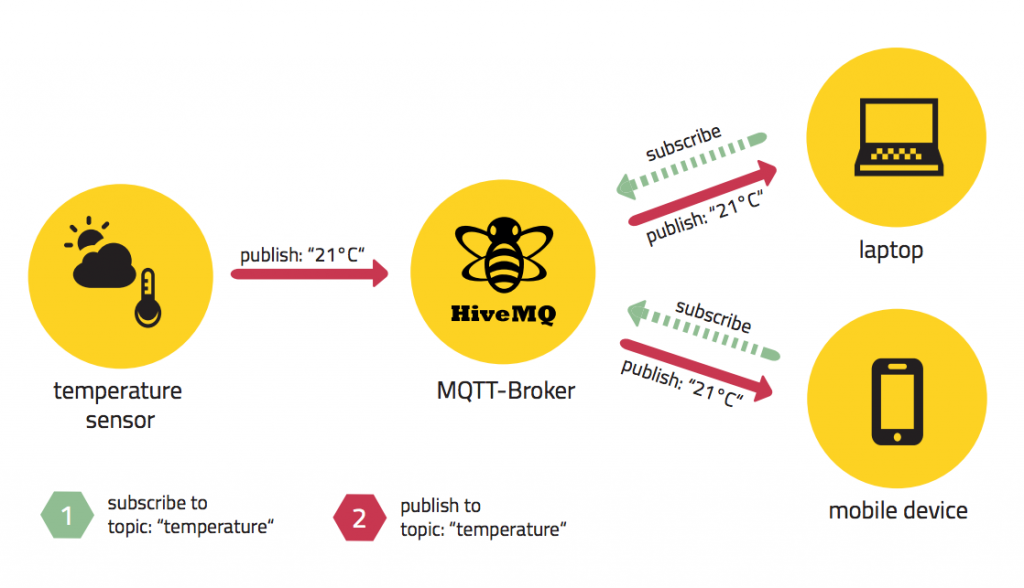
\includegraphics[width=0.7\textwidth]{img/mqtt-basics-by_hivemq.png}
	\caption{Schaubild zum Publish- / Subscribe-Vorgang in MQTT Quelle: \cite{hivemq.com-mqtt-essentials-publish-subscribe}}
	\label{fig:pubsub-example}
\end{figure}
Das obige Bild (\ref{fig:pubsub-example}) zeigt wie Clients (egal ob publizierende oder abonnierende) mit dem Broker eine Verbindung haben. Die beiden Abonnenten auf der rechten Seite interessieren sich für die Temperatur und müssen im Programmcode einen so genannten Callback / Listener an die Subscription anhängen. Sobald der Client auf der linken Seite im Bild nun wie in diesem Beispiel die Temperatur-Daten bereitstellt (publiziert), wird der Broker diese an die angemeldeten beiden Abonnenten zustellen.

\section{Ausführung der fertigen Artefakte}
Die fertigen Artefakte (die Jars) der Services, die aus dem Maven-Prozess rauskommen lassen sich auf dem Ubuntu-Linux des Roboters einfach als System-Dienst über den SystemD starten. Dazu wird pro auszuführenden Service eine Datei mit folgendem Inhalt hingelegt:
\begin{lstlisting}
$ cat cat /etc/systemd/system/robocup-<name>.service 
[Unit]
Description=LiDAR microservice
Requires=mosquitto.service
After=network.target mosquitto.service

[Service]
ExecStart=/usr/bin/java -jar /usr/share/robocup/positioning/robocup-lidar-service-20180612-jar-with-dependencies.jar

[Install]
WantedBy=multi-user.target
\end{lstlisting}

Für die Linux-Einsteiger könnten nachfolgende Befehle aus Tabelle \ref{tab:linuxCommands} nützlich sein.
\begin{table}[H]
	\centering
	\begin{tabular}{p{7cm}p{8cm}} \toprule
	\textbf{Befehl}					& \textbf{Beschreibung}						\\ \midrule
	\texttt{systemctl daemon-reload}		& Die Dateien im Ordner \ctexttt{/etc/systemd/system/..} neu einlesen nach dem Bearbeiten.\\ \midrule
	\texttt{systemctl status <name>.service}	& Status anzeigen						\\ \midrule
	\texttt{systemctl enable <name>.service} 	& Autostart aktivieren						\\ \midrule
	\texttt{systemctl disable <name>.service} 	& Autostart deaktivieren					\\ \midrule
	\texttt{systemctl start <name>.service} 	& Dienst starten						\\ \midrule
	\texttt{systemctl stop <name>.service} 		& Dienst beenden						\\ \midrule
	\texttt{journalctl -f -u <name>.service} 	& Logs zu einem Dienst anzeigen. Der Parameter \ctexttt{-f} behält die Datei offen und zeigt kontinuierlich (live) neue Logzeilen an.\\ \bottomrule
	\end{tabular}
	\caption{Nützliche Linux-Befehle}
	\label{tab:linuxCommands}
\end{table}
